\documentclass[12pt]{article}
\usepackage{amsmath}
\usepackage{mathtools}
\usepackage{bigints}
\usepackage{parskip}
\usepackage{amssymb}
\usepackage{relsize}
\usepackage{fullpage}
% \DeclareMathSizes{12}{17.28}{9}{7} % (a)

\DeclareMathSizes{12}{17.28}{12}{12} % (a)


\usepackage{hyperref}



	\addtolength{\topmargin}{-.5in}
	\addtolength{\textheight}{1.75in}



    \newenvironment{myindentpar}[1]%
     {\begin{list}{}%
             {\setlength{\leftmargin}{#1}}%
             \item[]%
     }
     {\end{list}}

\begin{document}
\title{College Algebra: Module 10 What You Need To Know}
\date{3-22-15}
\author{}
\maketitle

\section{Synthetic Division; the Remainder and Factor Theorems (Section 4.2)}


I will list some internet links because they can do a much better job explaining both of these methods than I can in here.

\textbf{Internet Links:}

\begin{itemize}
\item \href{https://www.youtube.com/watch?v=Ih1wb6AxhMI}{mathbff - Long Division} 

\item \href{https://www.youtube.com/watch?v=l6_ghhd7kwQ}{patrickJMT - Long Division}

\item \href{https://www.youtube.com/watch?v=FXgV9ySNusc}{Khan Academy - Long Division}

\end{itemize}

\textbf{Remainder Theorem:}

\begin{myindentpar}{1cm}

If a polynomial $p(x)$ is divided by $x-c$ using long division, the remainder is equal to $p(c)$
\end{myindentpar}

\textbf{Factor Theorem:}

\begin{myindentpar}{1cm}

For a polynomial $p(x)$

\begin{enumerate}

\item If $c$ is a zero of $p(x)$, then $x-c$ is a factor of $p(x)$
\item If $x-c$ is a factor of $p(x)$, then $c$ is a zero of $p(x)$ $\Big($i.e. $p(c) = 0\Big)$

\end{enumerate}

\end{myindentpar}

\section{The Zeroes of a Polynomial Function}

\textbf{Linear Factorization Theorem:}

\begin{myindentpar}{1cm}

If $p(x)$ is a polynomial function of degree $n \geq 1$, then $p$ has exactly $n$ linear factors and can be written in the form:
\newline

\centerline{$p(x) = a(x-c_{1}) \cdot (x - c_{2}) \cdots (x - c_{n})$}

\end{myindentpar}

\vspace{.5cm}

\textbf{Multiplicity of Zeroes} - if $p(x)$ is a polynomial function and $(x-c)$ occurs as a factor of $p(x)$ exactly $m$ times, then $c$ is called a zero of \textit{multiplicity} $m$

\newpage

\textbf{Conjugate Pairs Theorem:}

\begin{myindentpar}{1cm}

If $p(x)$ is a polynomial with real coefficients, complex zeroes must occur in conjugate pairs. That means, \textbf{if $a+bi$ is a zero, then $a-bi$ will also be a zero}
\end{myindentpar}

\section{Graphing Rational Functions (Section 4.5)}

\textbf{Vertical Asymptotes:} 

The line $x = a$ is a \textbf{vertical asymptote} for the graph of a function if $f(x)$ either increases or decreases without bound as $x$ approaches from either the right or left.  

\centerline{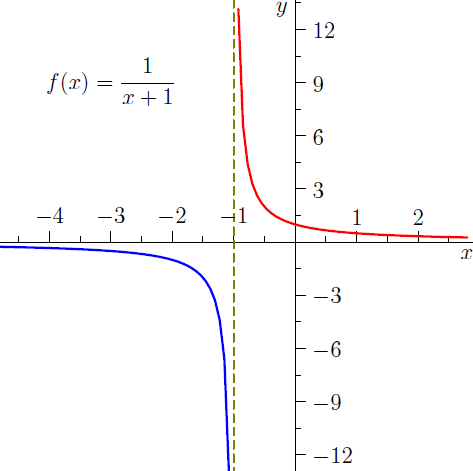
\includegraphics[scale = 0.5]{VerticalAsymptote.png}}

\textbf{Finding Vertical Asymptotes:} Set the denominator equal to $0$

\textbf{Horizontal Asymptotes:} 

The line $y = a$ is a \textbf{horizontal asymptote} for the graph of a function if $f(x)$ approaches $a$ as $x$ increases or decreases without bound

\centerline{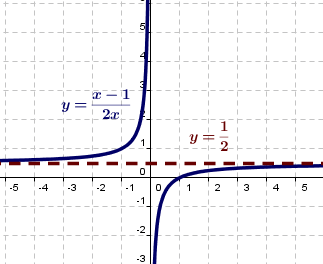
\includegraphics[scale = 0.7]{HorizontalAsymptote.png}}

\textbf{Finding Horizontall Asymptotes:} Compare the degree of the numerator and the degree of the denominator of a rational function. 

\begin{enumerate}
\item Degree of Numerator $<$ Degree of Denominator $\implies y = 0$ is the horizontal asymptote
\item Degree of Numerator $=$ Degree of Denominator $\implies$ horizontal asymptote is the ratio of the leading coefficients in the numerator and denominator
\item Degree of Numerator $>$ Degree of Denominator $\implies$ there is no horizontal asymptote
\end{enumerate}

\textbf{Steps to Graphing Rational Functions: $R(x) = \dfrac{N(x)}{D(x)}$}

\begin{enumerate}

\item Find the y-intercept, $R(0)$, if it exists
\item Find the zeroes of $R(x)$ by setting the numerator $N(x) = 0$
\item Find the vertical asymptotes. In other words, find the zeroes of $D(x)$
\item Find the horizontal asymptote, if it exists
\item Determine if the graph will cross the horizontal asymptote
\item Compute any additional points needed to sketch the graph

\end{enumerate}

\section{Polynomial and Rational Inequalities (Section 4.6)}

\textbf{Steps to Solving a Polynomial Inequality:} 

\begin{enumerate}

\item Move every term to one side of the inequality
\item Find the zeroes of the resulting polynomial
\item Drawn a number line and plot the zeroes from step 2
\item Test points \textbf{inside} each interval to see if the function is positive or negative
\item See which interval(s) make the inequality true

\end{enumerate}

(See handwritten notes on Polynomial Inequalities on Icon)

\vspace{.5cm}

\textbf{Steps to Solving a Rational Inequality:} 

\begin{enumerate}

\item Move every term to one side of the inequality
\item Put everything over a common denominator
\item Find the points where the function is undefined by setting the denominator equal to $0$ and solving
\item Ignore the  denominator and set only the numerator equal to $0$ to find the points where the function is equal to $0$
\item Draw a number line and plot the points where the function is undefined \textbf{and} where the function is $0$
\item Test points \textbf{inside} each interval to see if the function is positive or negative
\item See which interval(s) make the inequality true

\end{enumerate}

(See handwritten notes on Rational Inequalities on Icon)
















































\end{document}